\documentclass[12pt,a4paper]{article}
\usepackage[utf8]{inputenc}
\usepackage[T1]{fontenc}


\usepackage{amsmath}
\usepackage{amssymb}

\usepackage{lmodern}
\usepackage{indentfirst}
\usepackage{hyperref}
\usepackage{float}

\usepackage{enumitem}

\usepackage{graphicx}
\graphicspath{ {/} }

\begin{document}


\begin{titlepage}
	\centering
	\par\vspace{1cm}
	{\scshape\LARGE Kvantovo-chemické výpočty \par}
	\vspace{1cm}

	{\huge\bfseries Návrh  \par}
	\vspace{2cm}
	{\Large\itshape Jaroslav Ištok \par}
	{\Large\itshape Katarína Fabianová \par}
	{\Large\itshape Dušan Suja \par}
	{\Large\itshape Jerguš Adamec \par}
	\vfill
	{\large \today\par}
\end{titlepage}

\pagebreak

\tableofcontents

\pagebreak



\section{Diagramy}

\subsection{Entitno-relačný diagram}

\begin{figure}[H]
	\caption{Entitno - relačný diagram}
	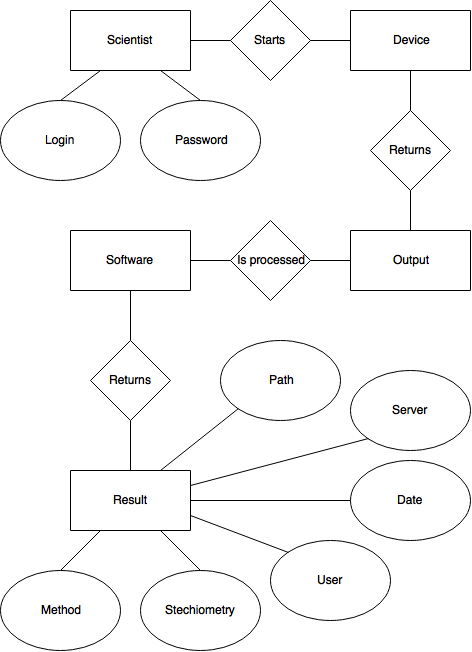
\includegraphics[width=\textwidth]{er_diagram}
	\label{fig:er_diagram}
\end{figure}
\ref{fig:er_diagram}
Entitno-relačný diagram znázorňuje vzťahy (relácie) medzi entitami. Diagram je použitý na modelovanie priestoru domény, pre ktorú sa informačný systém vyvíja (ústav experimentálnej fyziky). Entity sú zakreslené do obdĺžnikov. Vzťahy (relácie) medzi entitami sú v kosoštvorcoch, sú prepojené so všetkými entitami, ktoré do daného vzťahu vstupujú a sú pomenované. Entity majú svoje atribúty, ktoré sú do diagramu zakreslené ako ovály spojené so svojou entitou úsečkou.

\subsection{Use case diagram}
\begin{figure}[H]
	\caption{Use case diagram}
	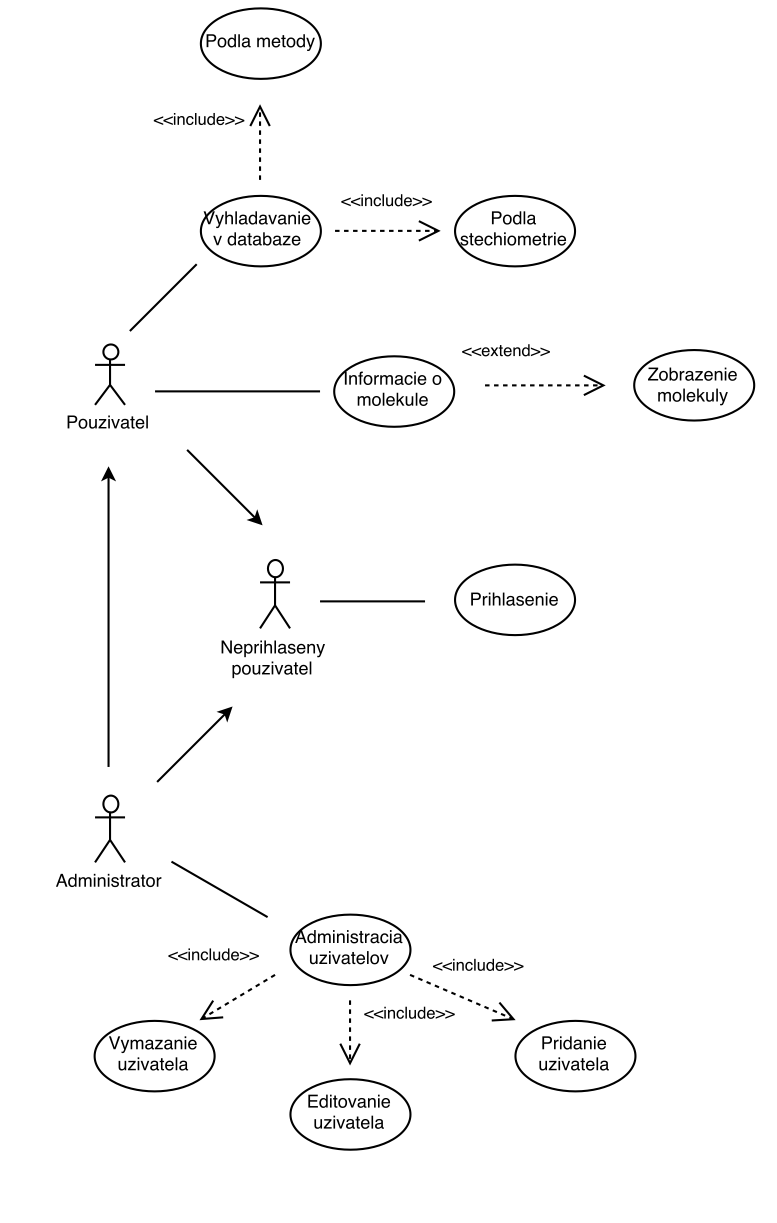
\includegraphics[width=\textwidth]{use-case}
	\label{fig:use_case}
\end{figure}

\ref{fig:use_case}
Use case diagram popisuje interakciu používateľov (aktorov) s aplikáciou. Neprihlásený používateľ sa môže prihlásiť. Prihlásený používateľ môže robiť administračné úkony ako napríklad: vymazávať, editovať alebo pridávať nových používateľov. Ďalej môže vyhľadávať v databáze výsledkov meraní podľa rôznych kritérii, či zobraziť výpis podrobných informácii o danej molekuje a tiež zobraziť jej náhľad.

\subsection{Stavový diagramy}
\begin{figure}[H]
	\caption{Stavový diagram}
	\includegraphics[width=\textwidth]{state}
	\label{fig:state}
\end{figure}

\ref{fig:state}
Stavový diagram popisuje proces spracovania súboru aplikáciou. Spracovanie sa začína otvorením súboru a jeho následnou prvotnou analýzou (validáciou). V prípade, že súbor nie je validný, tak sa nepokračuje ďalej v jeho spracovaní. V prípade, že súbor je validný sa zistí, či má súbor windowsový alebo linuxový formát. Tieto 2 formáty sa líšia vnútornou štruktúrou a teda aj spôsobom spracovania. Zo súboru sa následne vyparsujú potrebné dáta a spracovanie súboru skončí jeho zatvorením. 

\subsection{Sekvenčný diagram - spracovanie súboru}
\begin{figure}[H]
	\caption{Sekvenčný diagram - spracovanie súboru}
	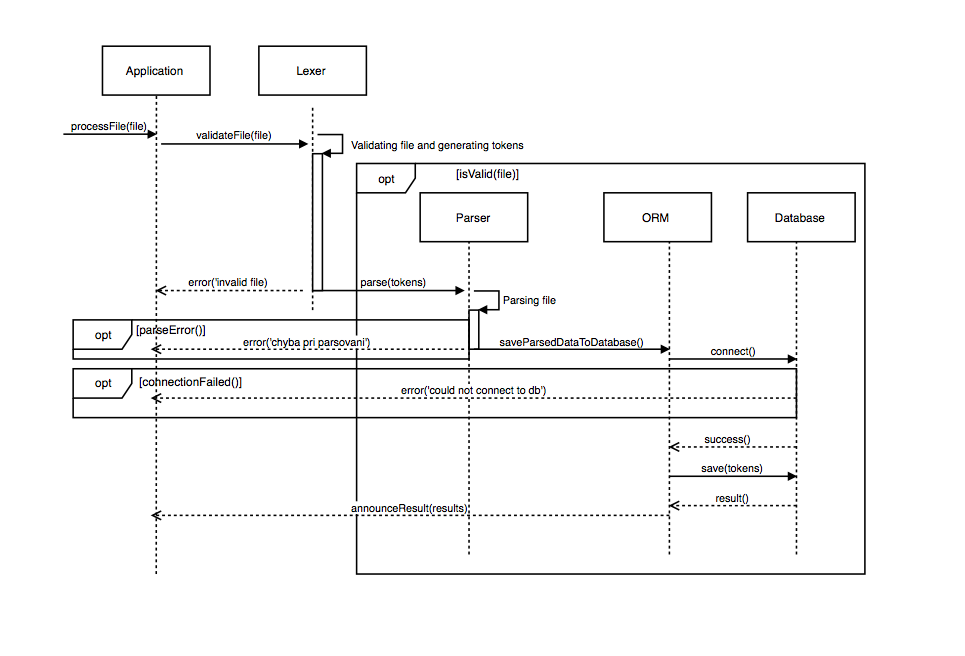
\includegraphics[width=\textwidth]{sequence_file}
	\label{fig:seq}
\end{figure}

\ref{fig:seq}
Diagram popisuje komunikáciu komponentov našej aplikácie počas spracovania súboru. Na začiatku aplikácia pošle lexeru požiadavku na validáciu súboru. Lexer súbor zvaliduje a rozparsuje na tokeny, v prípade chyby, pošle hlavnému programu správu s chybou. Tokeny pošle parseru, ktorý ich rozparsuje. Dáta z parseru sa pošlú ORM-ku, ktoré sa pripojí k databáze a uloží do nej naparsované dáta. Na konci pošle správu o úspechu, resp. neúspechu celej operácie do hlavného programu, ktorý ju spracuje.

\subsection{Sekvenčný diagram -  pripojenie k databáze}
\begin{figure}[H]
	\caption{Sekvenčný diagram - pripojenie k databáze}
	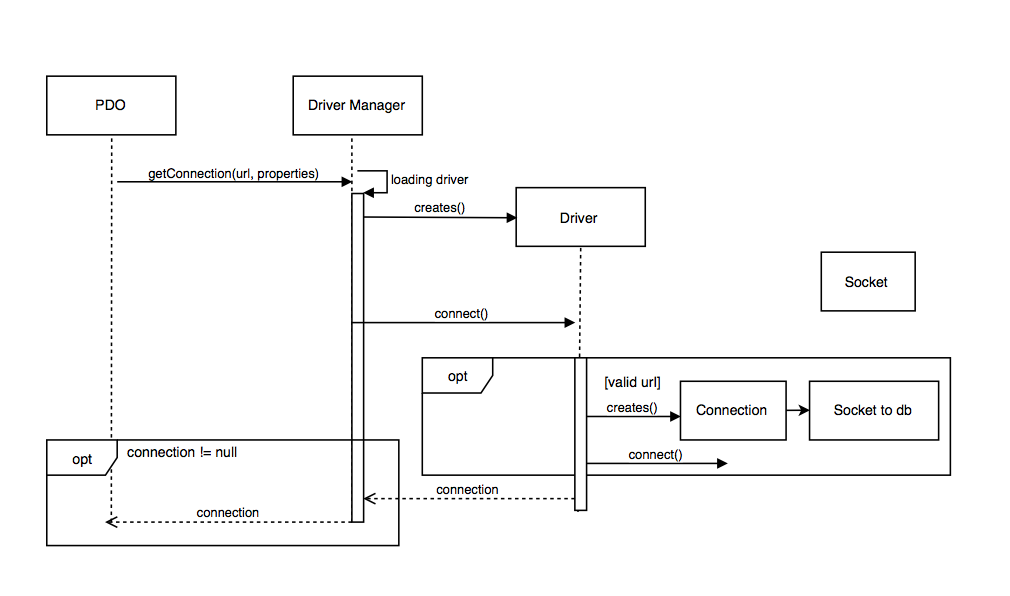
\includegraphics[width=\textwidth]{db}
	\label{fig:db}
\end{figure}

\ref{fig:db}
Diagram popisuje proces pripojenia k databáze. Knižnica PDO pošle požiadavku na získanie spojenia k databáze driver manageru. Ten načíta drivre, vyberie správny a vytvorí jeho inštanciu. Driver sa následne pokúsi vytvoriť spojenie k databáze, tým, že sa pokúsi pripojť na socket. V prípade neúspechu sa pošle správa do PDO o neúspechu. V prípade úspešného pripojenia na socket sa vráti spojenie k databáze do PDO.

\subsection{Triedny diagram}
\begin{figure}[H]
	\caption{Triedny diagram}
	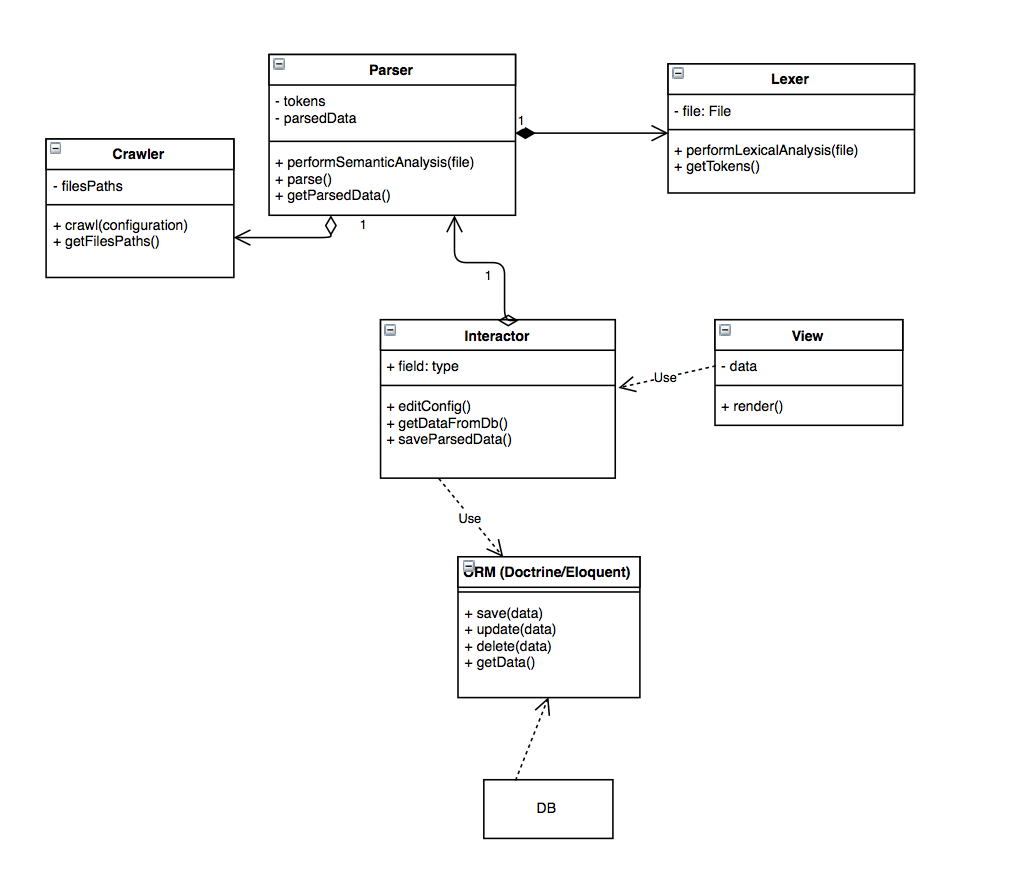
\includegraphics[width=\textwidth]{class_diagram}
	\label{fig:class_diagram}
\end{figure}

\ref{fig:class_diagram}
Triedny diagram modeluje jednotlivé triedy a vzťahu medzi nimi. Každá entita triedneho diagramu popisuje triedu a jej základné atribúty a metódy. Medzi triedami sú šípky, ktoré reprezenutujú jednotlivé vzťahy. Parser bude používať Crawler na vyhľadanie súborov a rovanko bude pouívať aj Lexer, pomou ktorého spraví lexikálnu analýzu súboru. Interactor bude akési spojítko jednotlivých hlavných častí aplikácie. View-u bude poskytovať dáta na zobrazenie a Parseru poskytne prístup k databáze.


\subsection{Dátový model databázy}
\begin{figure}	[H]
	\caption{Dátový model}
	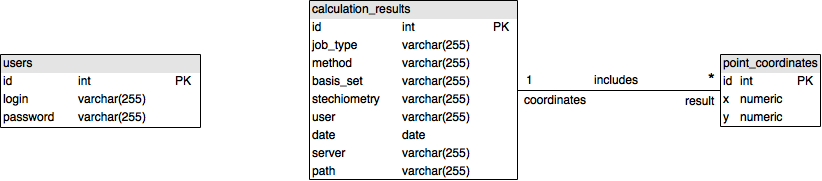
\includegraphics[width=\textwidth]{datovy_model}
	\label{fig:datovy_model}
\end{figure}

\ref{fig:datovy_model}
Dátový model popisuje štruktúru databázy
\subsubsection*{Users}
Tabuľka users obsahuje zoznam používateľov. Používatelia majú priradené id, plniace funkciu primárneho kľúča (user id), meno, pod ktorým sa prihlasujú (login) a heslo, s ktorým sa prihlasujú (password).
\subsubsection*{Calculation results}
Tabuľka calculation results obsahuje zoznam výsledkov výpočtov. Výsledky výpočtov majú priradené id, plniace funkciu primárneho kľúča (calculation result id), spôsob testovania vzorky (job type), metódu testovania vzorky (method), iniciálnu konfiguráciu (basis set), zjednodušený chemický vzorec testovanej vzorky (stechiometry), používateľa, spúšťajúceho testovanie vzorky (user), dátum testovania vzorky (date), meno servera, ukladajúceho daný výsledok výpočtu (server) a cestu k súboru daného výsledku výpočtu (path).
\subsubsection*{Point coordinates}
Tabuľka point coordinates obsahuje zoznam súradníc bodov. Súradnice bodov majú priradené id, plniace funkciu primárneho kľúča (point coordinate id), súradnicu x bodu (x), súradnicu y bodu (y) a id, plniace funkciu cudzieho kľúča (calculation result id).
\subsubsection*{Popis vzťahov}
Tabuľka users sa neviaže na žiadnu tabuľku. Tabuľka point coordinates sa viaže na tabuľku calculation results tak, že jedna súradnica bodu je obsiahnutá v práve jednom výsledku výpočtu, pričom jeden výsledok výpočtu môže obsahovať niekoľko súradníc bodov.


\subsection{Dekompozícia}
Komponent Autorizacia
Pomocou tohto komponentu sa bud mc pouvatelia sprvnym vyplnenm prihlaso- vacieho formulra prihlsi do systmu. Komponent budu vyuzivat bezny pouzi- vatelia aj pouzivatelia s administratorskymi pravami. Udaje z formulara sa porovnaju s udajmi v databaze. Pri zhode sa pouvate prihlsi do systmu a poda typu tu ma k dispozci rzne funkcionality systmu.
Komponent Crawler
Komponent bude vyhladavat subory s vysledkami vypoctov z meracich pristro- jov, ktore su ulozene nakonkretnych serveroch.
Komponent Spracovanie suboru
Tento komponent z analyzuje (zisti ci subory maju validnu strukturu) a nasledne spracuje vyhladane subory do vhodneho formatu.
Komponent Databaza
Komponent, ktory ma na starosti pripojenie a pracu s databazou.

\section{Návrh používateľského rozhrania rozhranie}
\begin{figure}[H]
	\caption{Používateľské rozhranie 1}
	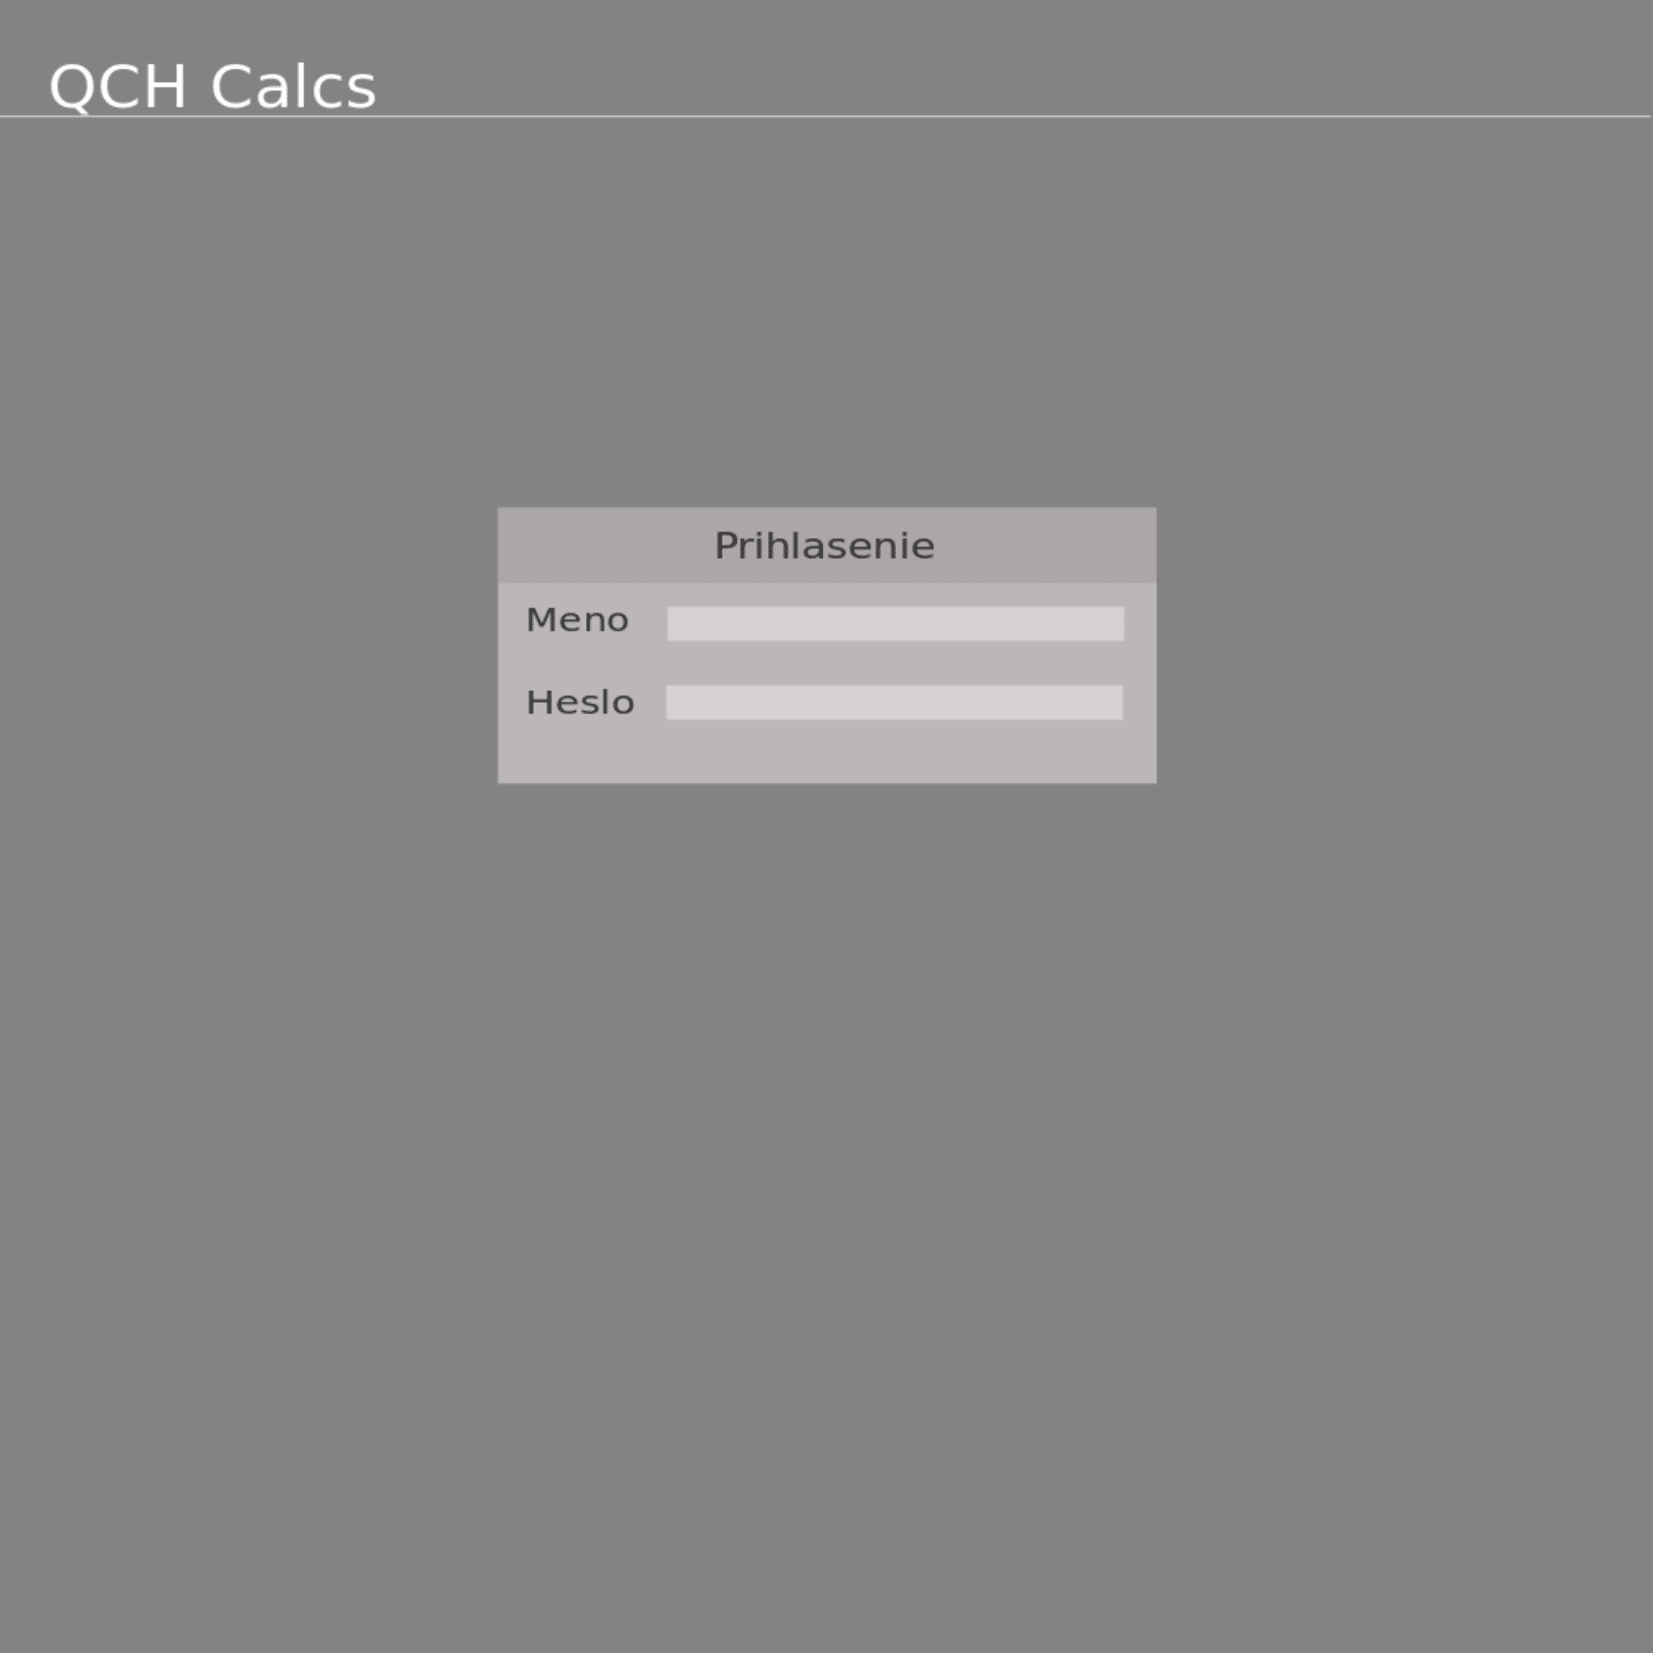
\includegraphics[width=\textwidth]{dizajn-1}
	\label{fig:ui1}
\end{figure}

\begin{figure}[H]
	\caption{Používateľské rozhranie 2}
	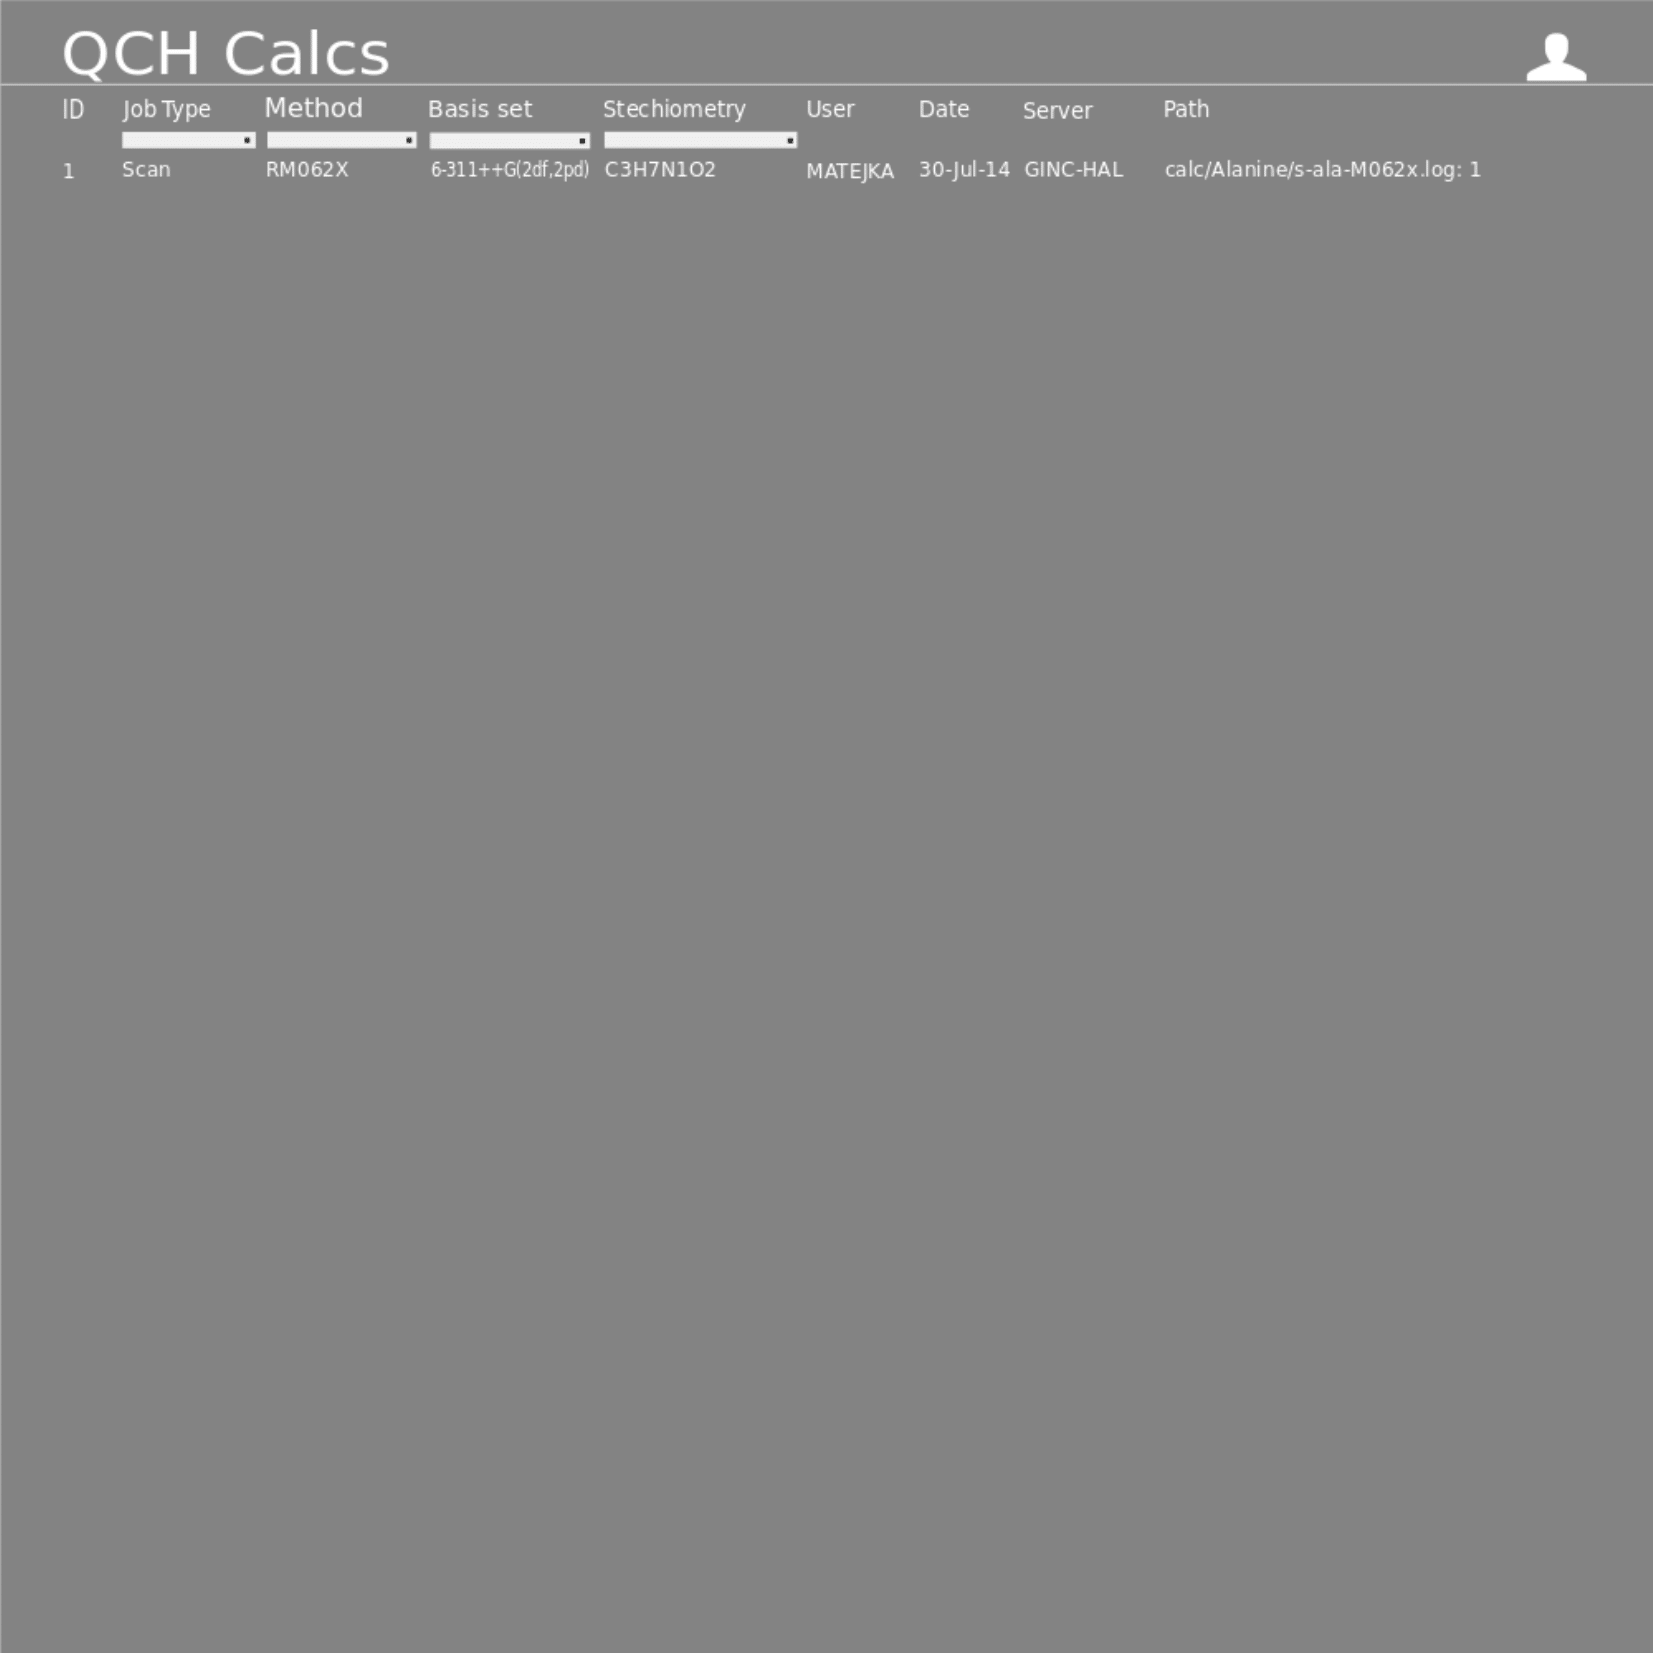
\includegraphics[width=\textwidth]{dizajn-2}
	\label{fig:ui2}
\end{figure}[H]

\begin{figure}[H]
	\caption{Používateľské rozhranie 3}
	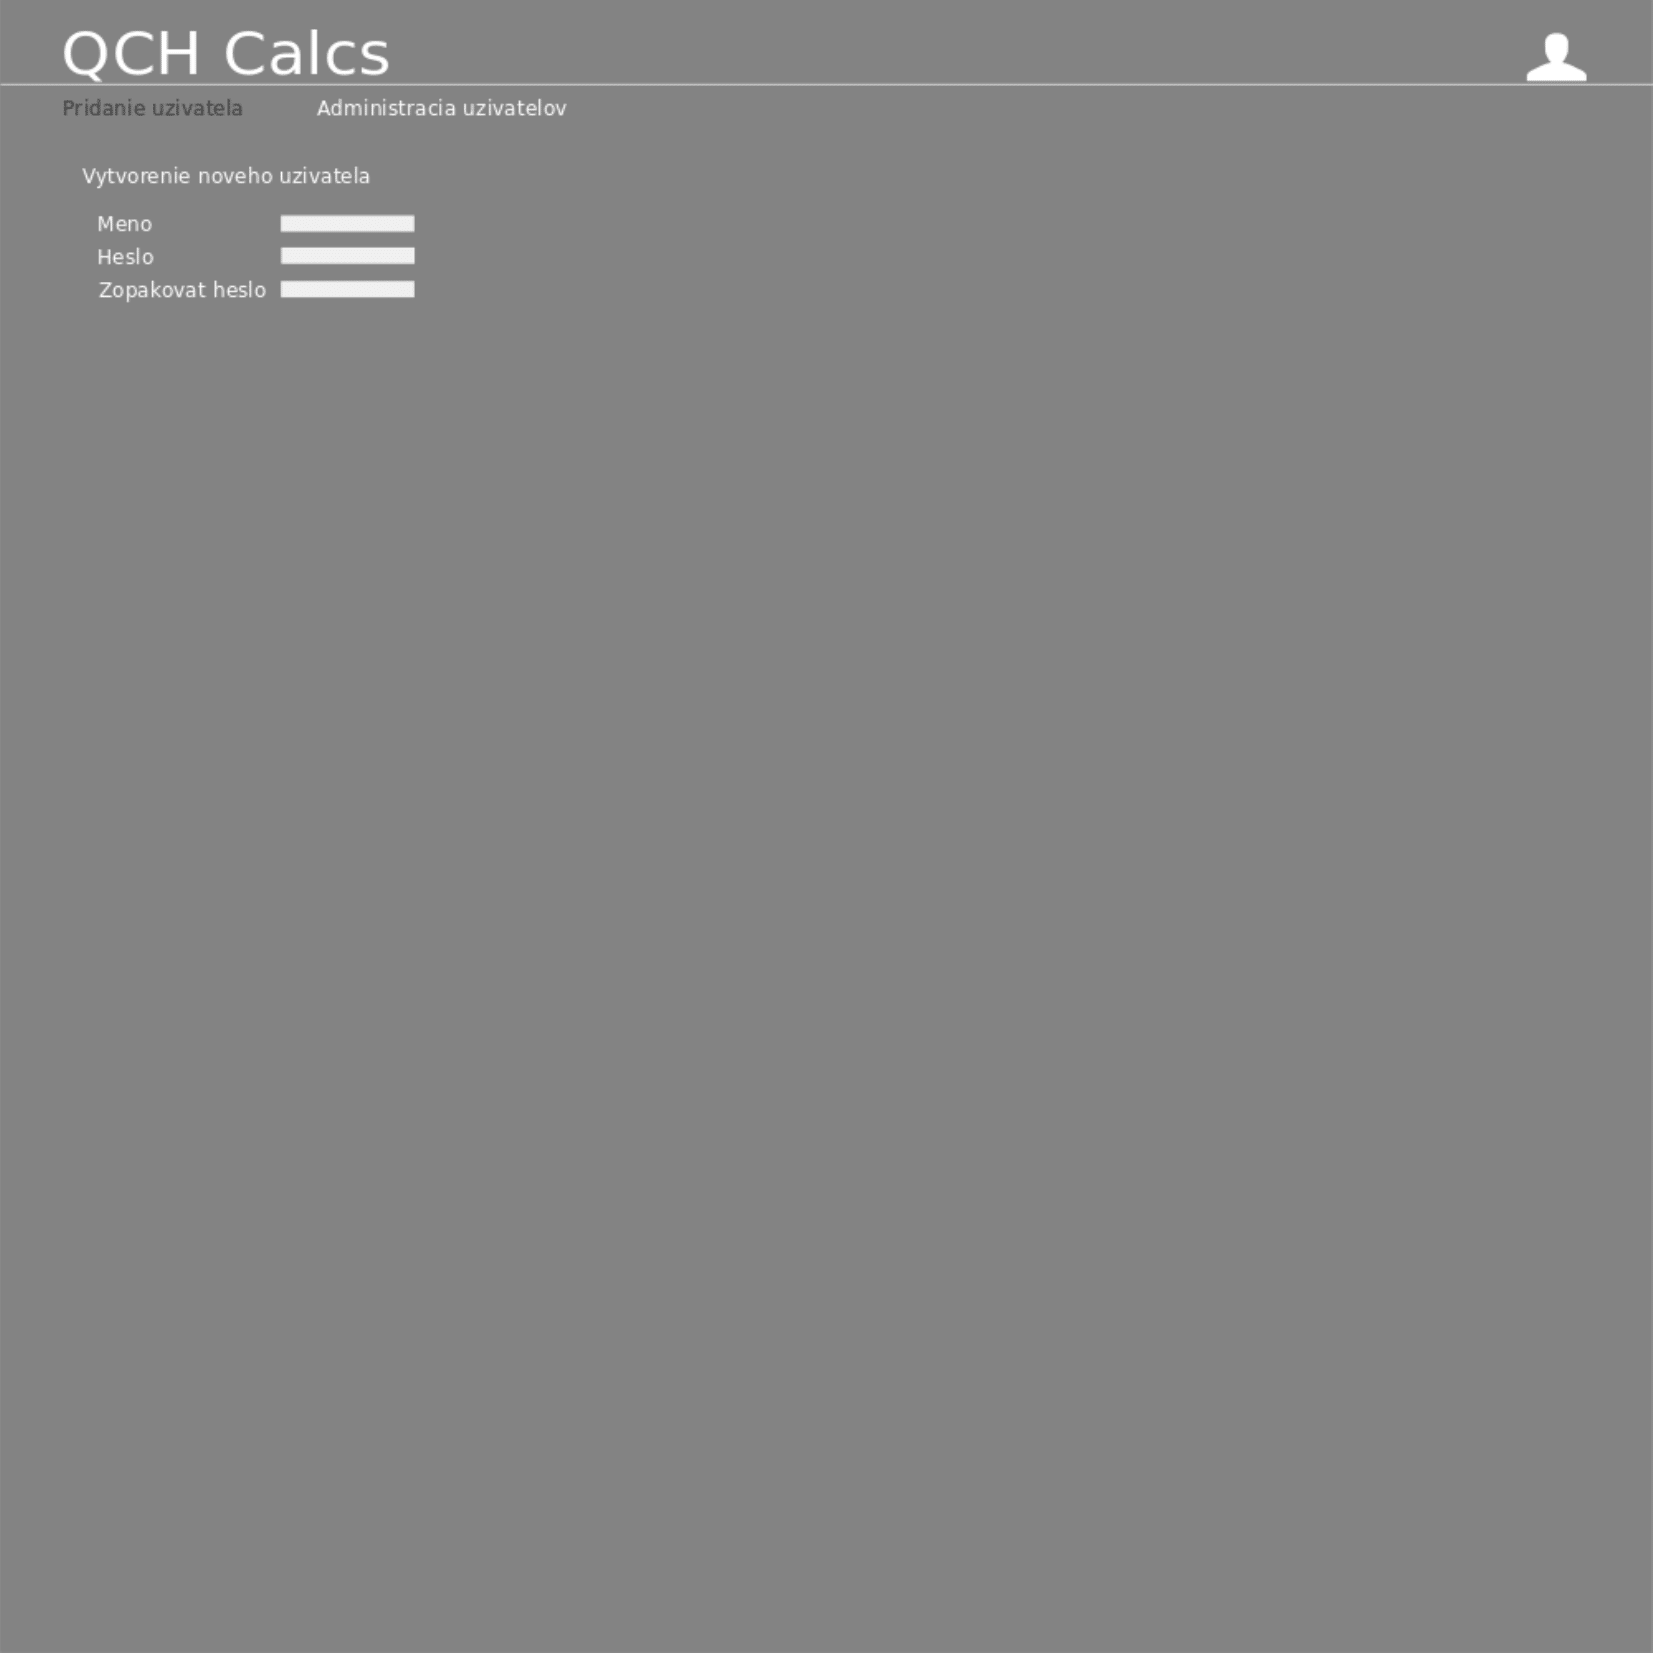
\includegraphics[width=\textwidth]{dizajn-3}
	\label{fig:ui3}
\end{figure}

\ref{fig:ui1}
Používateľké rozhranie aplikácie bolo navrhnuté jednoducho podľa požiadaviek zadávateľa projektu.

\section{Analýza technológii}
\subsection{Výber programovacieho jazyka}
Pri výbere programovacieho jazyka sme sa rozhodovali medzi Python-om a PHP. 
Vybrali sme si PHP, pretože je pre tento projekt najvhodnejší, medzi výhody, ktoré nám ponúka pri vývoji patria napríklad:
\begin{itemize}
	\item Patrí medzi najpoužívanejšie jazyky vo webových aplikáciach
	\item Je predinštalovaný na serveri, na ktorom bude bežať aj naša aplikácia
	\item Plne podporuje objektovo orientované programovanie
	\item V PHP je na výber veľa kvalitných frameworkov na prácu s databázou
	\item Vieme s ním efektívne pracovať
\end{itemize}
Python je náročnejšie nakonfigurovať na webovom serveri, kde pravdepodobne nebudeme mať možnosť inštalácie nového softwéru a oproti PHP ponúka len málo výhod pre náš projekt. Žiadnu podstatnú výhodu nám Python neponúka.

\subsection{Výber databázového systému}
Pri výbere databázového systému sme sa rozhodovali medzi Mysql a PostgreSql. PostgreSql ponúka veľa pokročilých funkcii, ako napríklad rekurzívne dopyty, pohľady. Naša aplikácia bude obsahovať jednoduchú databázu s malým počtom tabuliek a tieto pokročilé funkcie nevyužijeme. Preto sme si vybrali mysql databázu, ktorá je predinštalovaná na serveri a jej databázové enginy sú optimalizované pre webové aplikcie.


\section{Testovacie scenáre}
\subsection{Existencia súboru}
Otestovať existenciu súboru a jeho korektné otvorenie. Ak funkcia dosta\-ne cestu korektného súboru, so súborom sa dá ďalej pokračovať, v opačnom prípade funkcia súbor zahodí a nepokračuje sa v ďalšom spracovávaní.

\subsection{Crawler}
Otestovať funkcionalitu Crawlera. Používateľ pridá nové súbory v používateľskom rozhraní. Crawler má nájsť novopridané súbory a aktualizovať databázu. 

\subsection{Validnosť súboru}
Otestovať validitu súboru. Ak funkcia dostane validný súbor (je v požado\-vanom formáte), pokračuje sa ďalej v procese. V opačnom prípade ak funkcia dostane nevalidný vstup (súbor je v zlom formáte), ďalej sa nepokračuje a funkcia súbor zahodí.

\subsection{Rozlišovanie linuxových a windowsových súborov}
Otestovať rozlišovanie medzi linuxovým a windowsovým súborom (rozdiel je v type súboru a v pár znakoch). Funkcia rozlíši, či dostala na vstup linu\-xový alebo windowsový súbor a následne sa súbor parsuje podľa linuxového alebo windowsového formátu.  

\subsection{Databáza}
Otestovať pridávanie nových prvkov do databázy. Pridá sa nový korektný súbor a následne treba zistiť, či sa pridal aj do databázy. Pridá sa nový nekorektný súbor, následne treba skontrolovať, či sa údaje zo súboru nepridali do databázy.

\end{document}

